\documentclass{beamer}

% Top-aligning columns within a top-aligned frame
% https://tex.stackexchange.com/questions/16447/beamer-top-aligning-columns-within-a-top-aligned-frame
\makeatletter
\newenvironment{myitemize}{%
   \setlength{\topsep}{0pt}
   \setlength{\partopsep}{0pt}
   \renewcommand*{\@listi}{\leftmargin\leftmargini \parsep\z@ \topsep\z@ \itemsep\z@}
   \let\@listI\@listi
   \itemize
}{\enditemize}
\makeatother  

\usepackage[USenglish]{babel}
\usepackage[utf8]{inputenc}
\usepackage{amssymb, amsmath}
\usepackage{bm}
\usepackage{color}
\usepackage{tikz}
\usepackage{url}
\hypersetup{
    colorlinks,
    citecolor=blue,
    filecolor=blue,
    linkcolor=blue,
    urlcolor=blue
}

\usetheme{Warsaw}
\setbeamertemplate{headline}{}
\newcommand*\oldmacro{}%
\let\oldmacro\insertshorttitle%
\renewcommand*\insertshorttitle{%
  \oldmacro\hfill%
  \insertframenumber\,/\,\inserttotalframenumber}
  

\bibliographystyle{apalike}
% make bibliography entries smaller
%\renewcommand\bibfont{\scriptsize}
% Now get rid of all the colours
\setbeamercolor*{bibliography entry title}{fg=black}
\setbeamercolor*{bibliography entry author}{fg=black}
\setbeamercolor*{bibliography entry location}{fg=black}
\setbeamercolor*{bibliography entry note}{fg=black}

% and kill the abominable icon
\setbeamertemplate{bibliography item}{}

\begin{document}
\title{Objects that sound }  
\subtitle{unsupervised localization of sources of sounds in images trained from videos}
\author{Radek Bartyzal}
\date{Date TBA} 
\institute{Let's talk ML in Prague}

\frame{\titlepage} 

\begin{frame}{Achievements}

Achievements:

\begin{itemize}

\item networks that can embed audio and visual inputs into a common space that is suitable for cross-modal retrieval
\medskip
\item network that can localize the object that sounds in an image, given the audio signal
\medskip
\item training from unlabelled video using only audio-visual correspondence (AVC) as the objective function. 
\end{itemize}
\medskip

\begin{block}{Cross-modal retrieval}
Use audio to search in an image.
\end{block}

\begin{block}{Self-supervision}
Labels are constructed directly from data.
\end{block}

\end{frame}
%--------- END Frame 1 -------------

\begin{frame}{Audio-visual correspondence (AVC)}

\begin{itemize}
\item[Input:] Pair of a video frame and 1 second of audio represented as a log-spectrogram.
\medskip
\item[Task:] Are they in correspondence or not?
\medskip
\item[Labels:] Obtained directly from video for both positives
(matching) and negatives (mismatched) pairs. 
\end{itemize}

\vfill

Learnt visual and audio representations are:
\begin{itemize}
\item discriminative = distinguish matched and mismatched pairs
\item semantically meaningful = network has to find semantical match between audio and an image (visual network has only 1 image as input)
\end{itemize}

\end{frame}
%--------- END Frame 1.5 -------------
\begin{frame}{Dataset}

\begin{itemize}
\item publicly available AudioSet dataset
\item 10 second clips from YouTube
\item authors filtered it for musical
instruments, singing and tools, yielding 110 audio classes
\item train set = 263k clips
\item validation set = 30k clips
\item test set = 4.3k clips
\item labels are only used for quantitative
evaluation purposes of cross-modal retrieval
\end{itemize}

\end{frame}
%--------- END Frame 2 -------------

\begin{frame}{Previous work - $L^3$}

$L^3$ = Look, Listen and Learn \cite{cit:l3}


\begin{enumerate}
\item Get embeddings by separate specialized sub-networks.
\item Concatenated embeddings go to fully connected layers that calculate the correspondence score.
\end{enumerate}



\vfill

Limitations:

\begin{itemize}
\item visual and audio representations are not aligned so they cannot be used for crossmodal retrieval - fixed by AVE-Net
\item cannot localize the sound source in an image - solved by AVOL-Net
\end{itemize}


\end{frame}
%--------- END Frame 3 -------------

\begin{frame}{Previous work - $L^3$}
\begin{figure}[h]
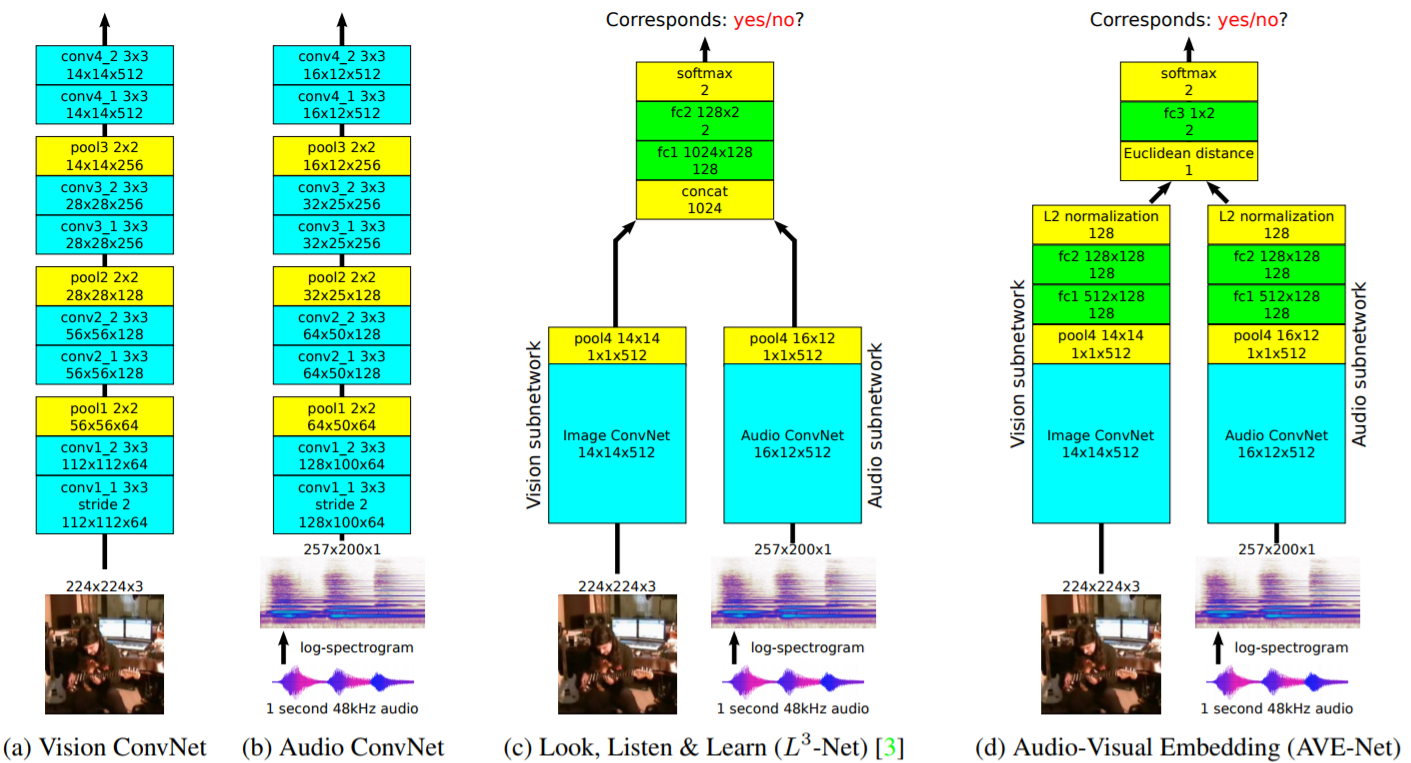
\includegraphics[width=\textwidth]{img/ave-net}
\caption{$L^3$ and AVE-Net descriptions.}
\end{figure}

\end{frame}
%--------- END Frame 4 -------------
\begin{frame}{Audio-Visual Embedding Network (AVE-Net)}
Changes compared to $L^3$:
\begin{enumerate}
\item fully connected layers are moved to the sub-networks
\item L2 normalization on top of them
\item 128-D embedding out of each sub-network
\item euclidean distance of the normalized embeddings
\item 1 layer followed by softmax 
\end{enumerate}

\vfill

The tiny FC layer scales and shifts the distance to
calibrate it for the subsequent softmax. The bias of the FC
essentially learns the threshold on the distance above which
the two features are deemed not to correspond.
\end{frame}
%--------- END Frame 5 -------------
\begin{frame}{Audio-Visual Embedding Network (AVE-Net)}

\begin{itemize}
\item The single
value that summarizes whether the image and the audio correspond,
forces the two embeddings to be aligned.
\item Use of the distance during training makes the features “aware” of the distance metric,
therefore making them amenable to retrieval.
\item Entire network trained from scratch.
\item Parameter-free euclidean distance.
\end{itemize}


\end{frame}
%--------- END Frame 6 -------------
\begin{frame}{Results}
\begin{block}{normalized discounted cumulative gain (nDCG)}
Measures quality of the ranked list of the top k retrieved items.
\end{block}

Each item in the test set is used as a query and the average \detokenize{nDCG@30} is reported.

\begin{figure}[h]
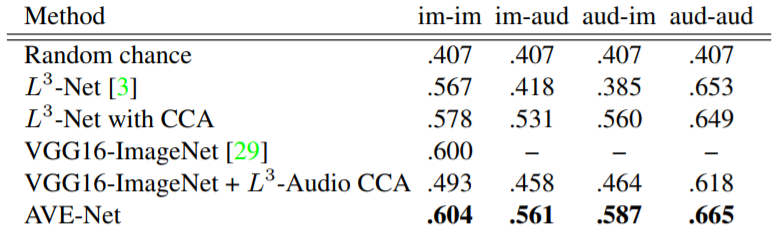
\includegraphics[width=\textwidth]{img/results}
\caption{"Our AVENet
beats all baselines convincingly." \cite{cit:ots} Yeah sure...}
\end{figure}

\end{frame}
%--------- END Frame 7 -------------
\begin{frame}{Extending the AVE-Net}

Extensions:
\begin{itemize}
\item use 25 frames instead of 1
\item add 10s of optical flow to the 1 frame
\end{itemize}

\vfill

Both had better performance on AVC task: 85\% vs AVE-Net 82\% vs $L^3$ 82\% but it does not translate into better crossmodal retrieval scores.

\end{frame}
%--------- END Frame 8 -------------
\begin{frame}{Audio-Visual Object Localization (AVOL-Net)}



\end{frame}
%--------- END Frame 9 -------------
\begin{frame}{Audio-Visual Object Localization (AVOL-Net)}

\end{frame}
%--------- END Frame 10 -------------
\begin{frame}{Results}

\end{frame}
%--------- END Frame 11 -------------
\begin{frame}{Sampling of negative pairs}

\begin{itemize}
\item Positive pair is a frame and one second of audio with the frame in the middle.
\item Videos have 25fps.
\item Positive audio samples start at multiples of 0.04s.
\item Getting a negative audio pair randomly allows the network to cheat. It recognizes that negative samples do not start at multiples of 0.04.
\item Cheating allowed 87.6\% vs correct 81.9\% at AVC task.
\item Solution = sample negative audio samples also at the multiples of 0.04.
\end{itemize}
 



\end{frame}

%--------- END Frame 12 -------------
\begin{frame}{Sources}

\begin{thebibliography}{0}

  \bibitem[1]{cit:ots} 1. Arandjelović, Relja, and Andrew Zisserman. "Objects that Sound." arXiv preprint arXiv:1712.06651 (2017). Accessible from: \url{https://arxiv.org/abs/1712.06651}
  
  \bibitem[2]{cit:l3} 2. Arandjelovic, Relja, and Andrew Zisserman. "Look, listen and learn." 2017 IEEE International Conference on Computer Vision (ICCV). IEEE, 2017. Accessible from: \url{https://arxiv.org/abs/1705.08168}
\end{thebibliography}
\end{frame}
 
 
 
\end{document}
